% Software License Agreement
%
% Author    Mike Purvis <MPurvis@clearpathrobotics.com>
% Copyright (c) 2018, Clearpath Robotics, Inc., All rights reserved.
%
% Redistribution and use in source and binary forms, with or without modification, is
% not permitted without the express permission of Clearpath Robotics.


\documentclass[]{clearpath-latex/clearpath-manual}
\graphicspath{{gen/}}
\usepackage{multirow}
\usepackage{gensymb}
\usepackage{dcolumn}
\usepackage{colortbl}
\usepackage{array}
\usepackage{needspace}



\begin{document}

\manualcover{cover-page.pdf}
\tableofcontents

\section{Introduction}
Clearpath Robotics Heron is a rugged and easy-to-use Unmanned Surface Vessel (USV) for research and rapid prototyping applications. This guide contains information about the setup, operation, and maintenance of your Heron USV.

\subsection{What's Included}

Included with each Heron are the following:

\begin{itemize}[nolistsep]
	\item 1x Clearpath Robotics Heron USV
	\item 1x 14.4V NiMH Battery Pack
	\item 1x Battery Pack Charger
	\item 1x Futaba Backup Remote Control (R/C)
\end{itemize}

Herons are often deployed with a Clearpath Long Range Wireless Network Station (sold separately). The Long Range Network Station includes:

\begin{itemize}[nolistsep]
	\item Clearpath Robotics Long Range Network Station
	\item Base Station Battery
	\item Base Station Battery Charger
\end{itemize}

\subsection{What's Required}

The embedded PC onboard Heron runs Ubuntu Linux 16.04 and ROS Kinetic. The development computer or laptop should be running the same operating system as the on-board computer; however, any version of Ubuntu supported by ROS Kinectic will work. If a laptop option was purchased with Heron it will already be configured with ROS and the appropriate ROS packages. For assistance setting up the development computer, please see the PC Setup section on page \pageref{pcsetup}.

Heron may also be driven using the included Futaba R/C controller as described in the Getting Started section on page \pageref{gettingstarted}. The R/C controller is intended as a backup to allow powered retrieval of Heron in case of a PC or network malfunction while on the water.

\section{The Basics}
This section provides an overview of the key specifications of the Heron platform. \autoref{h_the_basics1}, \autoref{h_the_basics2} and \autoref{h_the_basics3} give an overview of Heron's major components.

\begin{figure}[h]
  \centering  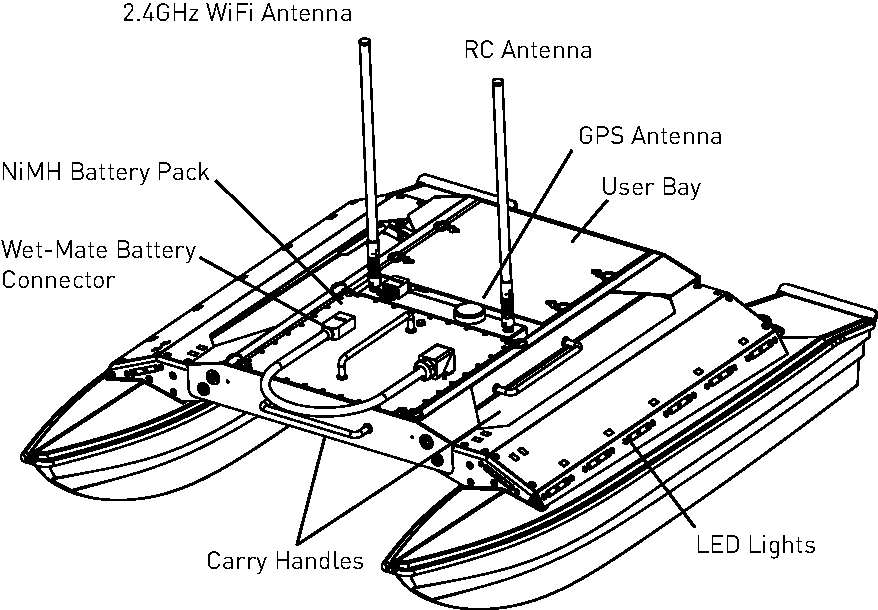
\includegraphics[width=0.75\linewidth]{graphics/basics_1.pdf}
  \caption{Heron at a Glance (actual boat may vary slightly from image shown)}
  \label{h_the_basics1}
\end{figure}

\begin{figure}[h]
  \centering  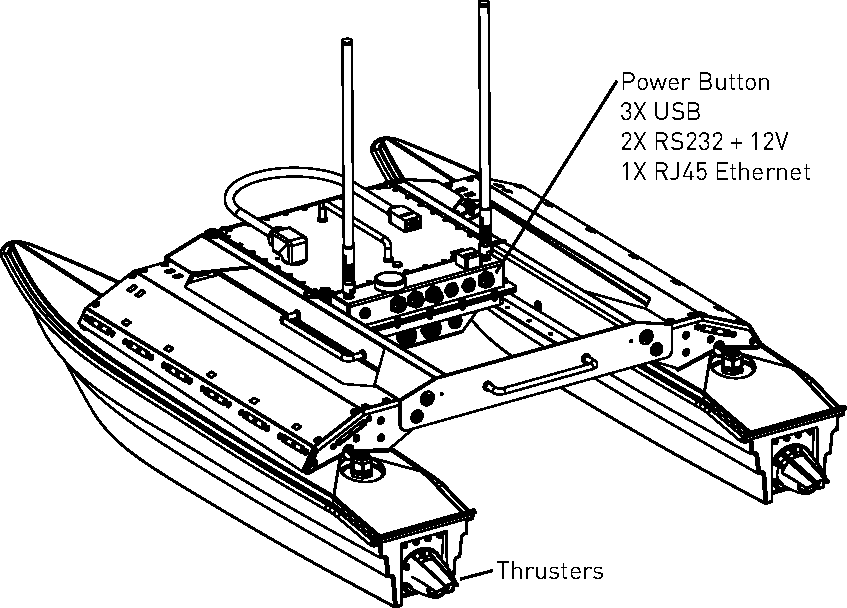
\includegraphics[width=0.75\linewidth]{graphics/basics_2.pdf}
  \caption{Heron at a Glance (actual boat may vary slightly from image shown)}
  \label{h_the_basics2}
\end{figure}

\begin{figure}[h]
  \centering  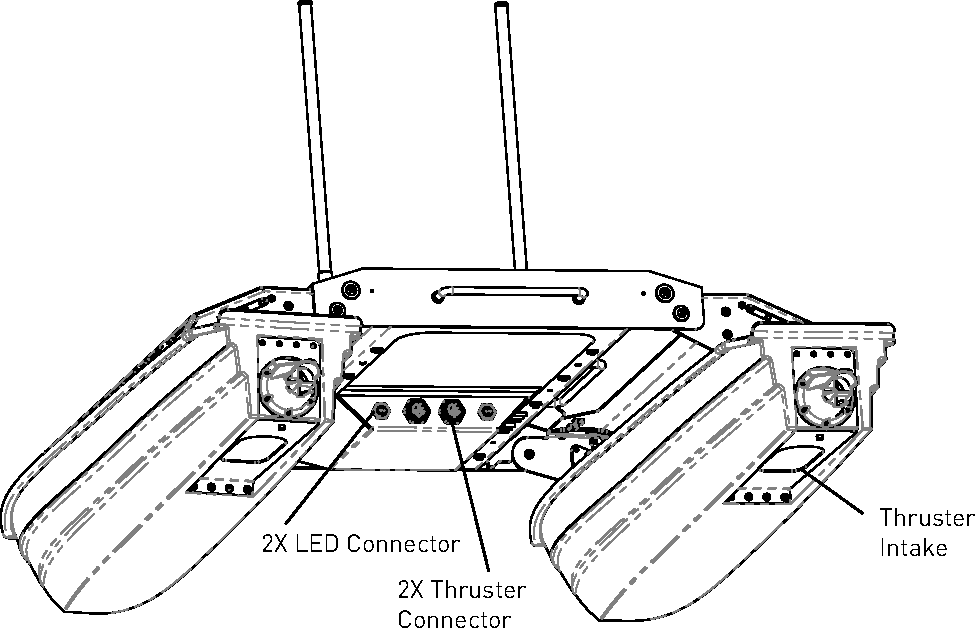
\includegraphics[width=0.75\linewidth]{graphics/basics_3.pdf}
  \caption{Heron at a Glance (actual boat may vary slightly from image shown)}
  \label{h_the_basics3}
\end{figure}

\newpage

\subsection{Hardware Architecture}
\autoref{h_architechure} gives an overview of the standard devices which make up Heron. This diagram is provided to aid the user in understanding the Heron system architecture.

\begin{figure}[h]
  \centering
  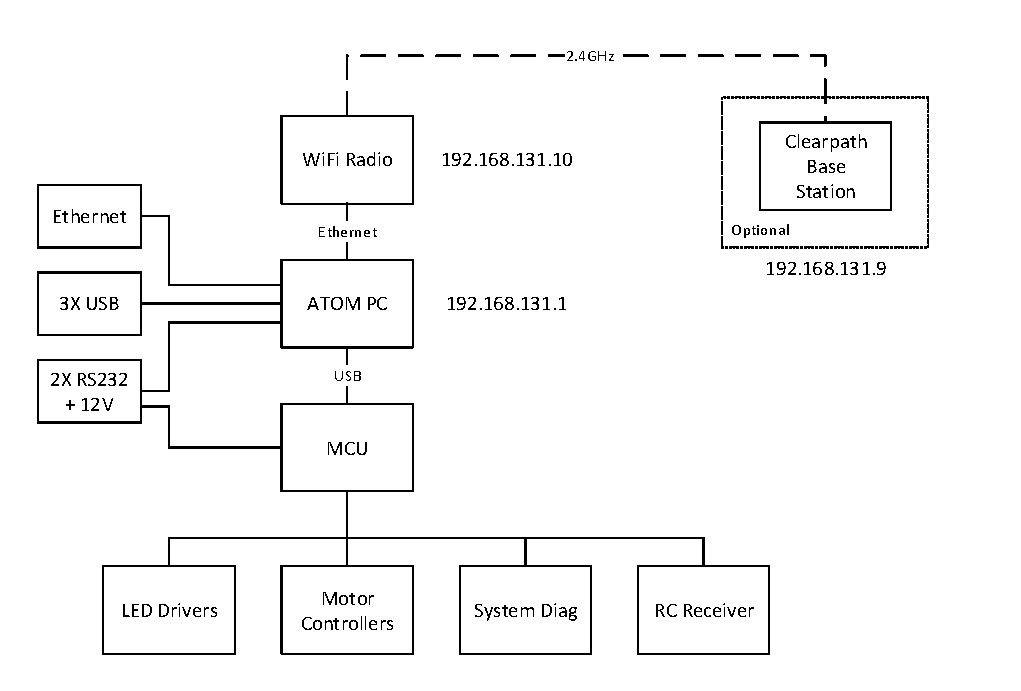
\includegraphics[width=0.85\linewidth]{graphics/h-architecture.pdf}
  \caption{Heron Architecture}
  \label{h_architechure}
\end{figure}


The eth0 interface is connected to a weatherproof connector in the User Payload Area. This connector is used to connect Ethernet payloads, such as an IP camera or LIDAR, but may also be used to connect to the vehicle over SSH, especially to adjust the wireless configuration (for example, to change the wireless password, or to associate with a different base station).
\newpage
\subsection{Status Indicators} \label{statusindicators}
The red and green running lights on the port and starboard sides of Heron indicate vehicle status based on the frequency and pattern of flashing. These patterns are described in \autoref{hstatusindicator}.

\bgroup
\def\arraystretch{1.5}%
\begin{table}[h]
\centering
\begin{tabular}{m{.25\textwidth} p{.6\textwidth}}
\rowcolor{lightgrey}
Light Pattern     & Description                                                                                                                                                                                              \\ \hline
Solid             & \textbf{No errors}. PC and wireless are active, and a command stream is being received and processed.                                                                                                             \\ \hline
Slow Single Pulse & \textbf{No command}. Indicates that the system is fully up, but the thrusters are not active due to an absence of command messages. Command messages must be sent at 10Hz or faster to maintain steady operation. \\ \hline
Slow Double Pulse & \textbf{Wireless Error}. Indicates that the onboard PC is unable to find the base station’s wireless network. If this indication is seen, check the battery level and indicator lights in the base station.       \\ \hline
Slow Triple Pulse & \textbf{Computer Error}. Indicates that the micro-controller in Heron cannot see the onboard PC. This is expected for about two minutes when first powering on, while the computer boots up.                  \\ \hline
Fast Single Pulse & \textbf{Manual Override}. Indicates that manual control by the Futaba R/C controller is active, and any commands originating from the PC will be disregarded.                                                     \\ \hline
Fast Double Pulse & \textbf{Critical Battery Pack}. Indicates that the system battery level is at or below 13V. Return to shore immediately. \\ \hline
\end{tabular}
\newline
\caption{Heron Status Indicators}
\label{hstatusindicator}
\end{table}
\egroup

The precedence order in the table is downward—that is, the bottom-most condition which is true will be what is indicated by the lights.

\newpage
\subsection{R/C Controller}
Heron ships with a Futaba R/C transmitter integrated as a means of backup control. The RC controller provides reliable long range control of the USV. Vehicle battery voltage is displayed on the controller if the boat is within range and is equipped with a Futaba Voltage Sensor.  It is recommended to remove all AA batteries and store them in a cool dry location when the R/C controller is not in use.

\begin{figure}[t]
  \centering
  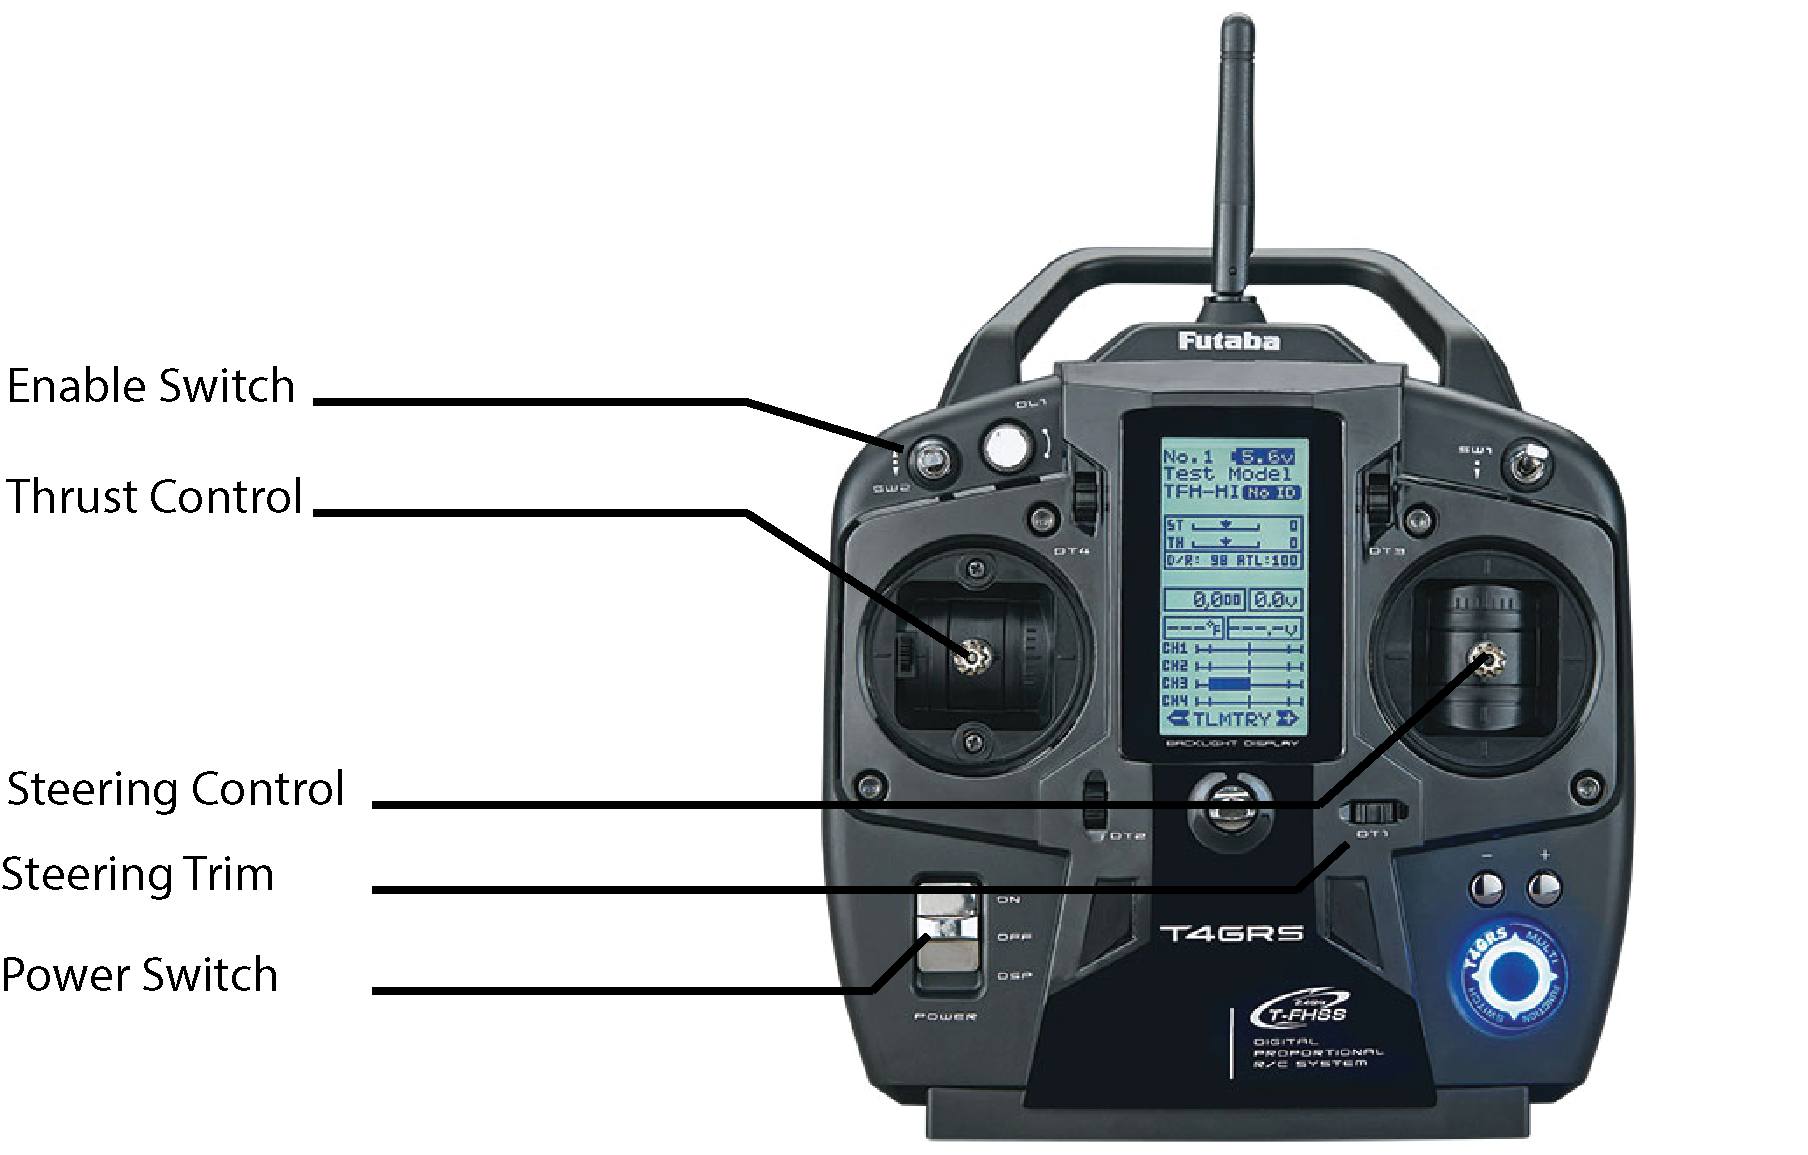
\includegraphics[width=0.85\linewidth]{graphics/h-futaba.png}
  \caption{Futaba R/C Transmitter}
  \label{h_futaba}
\end{figure}

Please see Backup R/C Operation on page \pageref{backupoperation} for details of operating Heron with the RC controller.

\newpage


\section{System Specifications}
Key specifications of Heron are shown in \autoref{systemspecs}.

\bgroup
\def\arraystretch{1.2}%
\begin{table}[h]
	\centering
	\begin{tabular}{>{\columncolor{lightgrey}}>{\raggedright}m{.25\textwidth} p{.25\textwidth} p{.25\textwidth}} \hline
	& 1300 mm length & 51.2 in length \\
	& 940 mm width & 37 in width \\
	\multirow{-3}{*}{Deployed Dimensions}
	& 340 mm height & 13.4 in height \\ \hline

	& 1300 mm length & 51.2 in length \\
	& 550 mm width & 21.6 in width \\
	\multirow{-3}{*}{Stowed Dimensions}
	& 340 mm height & 13.4 in height \\ \hline
	Chassis Weight (no battery) & 20 kg & 44 lbs \\ \hline
	Battery Weight & 9 kg & 20 lbs \\ \hline
	Draft & 150 mm & 5.9 in \\ \hline
	Maximum Payload & 10 kg & 22 lbs \\ \hline
	Rated speed (forward) & 1.7 m/s & 5.6 ft/s \\ \hline
	& 2.5 hours typical  \\
	\multirow{-2}{*}{Operating Time}
	& \multicolumn{2}{p{.5\textwidth}}{10 hours standby (no motion)} \\ \hline
	& 14.4V 29 Ah \\
	\multirow{-2}{*}{Battery Pack}
	& NiMH \\ \hline
	Battery Pack Charger & \multicolumn{2}{p{.5\textwidth}}{Short-circuit, over-current, over-voltage, and reverse voltage protection.} \\ \hline
	Charge Time & 10 hours \\ \hline
	User Power & \multicolumn{2}{p{.5\textwidth}}{12V fused at 2.5A} \\ \hline
	Communication & \multicolumn{2}{p{.5\textwidth}}{USB, TCP/IP, RS232} \\ \hline
	Standard Sensing & \multicolumn{2}{p{.5\textwidth}}{Battery Voltage, GPS, IMU} \\ \hline


	\end{tabular}
\newline
\caption{Heron System Specifications}
\label{systemspecs}
\end{table}
\egroup


\newpage

\section{Safety}
Clearpath Robotics is committed to the safety of our users. Please be advised that Heron is research equipment designed for prototyping applications and we are not able to protect operators, observers, and equipment from all possible use cases. This section provides guidelines to help ensure the safety of personnel and equipment, but the ultimate responsibility lies with the operator.

\subsection{General Warnings}
Heron is a rugged and high-performance vehicle. For the safety of yourself and others, conduct initial experiments in an area that is clear of obstacles and deeper than 0.6 m [24 in]. Although Heron is able to operate in very shallow water, this will avoid any possibility of running aground.

Indoor swimming pools provide an ideal environment for initial testing.

When starting out, it is recommended to favor slower speeds. Operating at speeds lower than 0.5 m/s will give the user more time to react if things don’t go quite as expected.

Adhere to all pool and open water safety considerations.

\begin{warning}
Never operate the Heron in a pool or other bodies of water while people are in the water.
\end{warning}

\subsection{Electrical System}
Heron is powered by a single 14.4V Nickel-Metal Hydride (NiMH) Battery Pack, the same battery chemistry found in many electric RC cars and boats. Please observe the following precautions:

\begin{itemize}[nolistsep]
	\item Do not tamper with the plug attached to the Battery Pack.
	\item Do not tamper with the Battery Pack connection on Heron.
	\item Do not operate Heron without the Battery Pack clamped securely in position.
	\item Do not tamper with the Electronics Bay.
	\item Charge the Battery Pack only with chargers provided by Clearpath Robotics.
\end{itemize}

\textbf{The Battery Pack has a rugged exterior to protect it from bumps and scrapes, but it still stores a large amount of electro-chemical energy and is inherently dangerous. Observe the above precautions carefully.}

\subsection{Lifting and Transport}
For the safety of users and to maximize the lifetime of Heron, please observe the following when manually transporting the robot:

\begin{itemize}[nolistsep]
	\item Heron should be lifted using only the two carrying handles on the vehicle itself.
	\item Ensure that Heron is powered off and the Battery Pack is removed when transporting longer distances.
\end{itemize}

\begin{warning}
Do not lift the vehicle from the battery pack handle! This may damage the battery retention inserts in the electronics enclosure
\end{warning}

\newpage

\section{Getting Started} \label{gettingstarted}
You are ready to go! This section details how to get the thrusters spinning.

\subsection{Platform Deployment}
Heron has been designed for easy deployment and rapid transit to and from work sites. The hulls and thrusters stow underneath the chassis to reduce the platform's overall size during transit. Unfolding the hulls is a tool-less operation, and is to be done prior to placing the platform in the water. Please see \autoref{h_pontoon} and the steps following.

\begin{figure}[h]
  \centering
  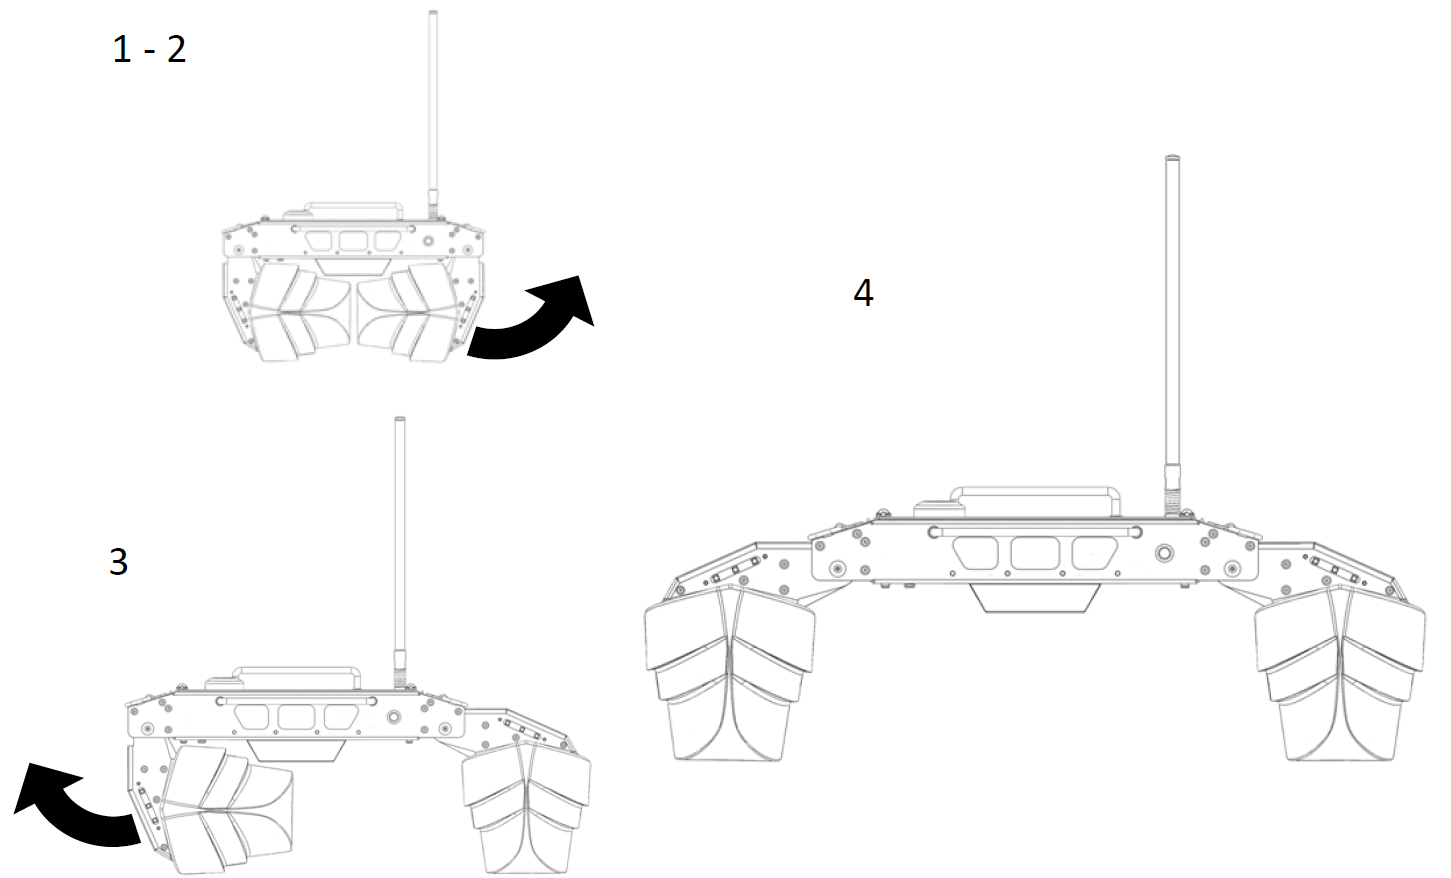
\includegraphics[width=0.75\linewidth]{graphics/kf_pontoon.png}
  \caption{Pontoon Deployment}
  \label{h_pontoon}
\end{figure}

\begin{enumerate}[nolistsep]
	\item Place stowed Heron right-side-up on the ground.
	\item Pull up a stowed hull to the deployment position, setting Heron back down afterward.
	\item Repeat this operation for the opposite hull.
	\item Heron is ready for battery installation and pre-launch check.
\end{enumerate}
\newpage

\subsection{Battery Pack Installation}
Heron comes with a Battery Pack that is discharged and disconnected for safety during shipping. Charge the battery prior to first time use.
To reconnect the Battery Pack, please see \autoref{h_batteryinstall} and the steps following.

\begin{warning}
Do not lift the vehicle from the battery pack handle! This may damage the battery retention inserts in the electronics enclosure
\end{warning}

\begin{figure}[h]
  \centering
  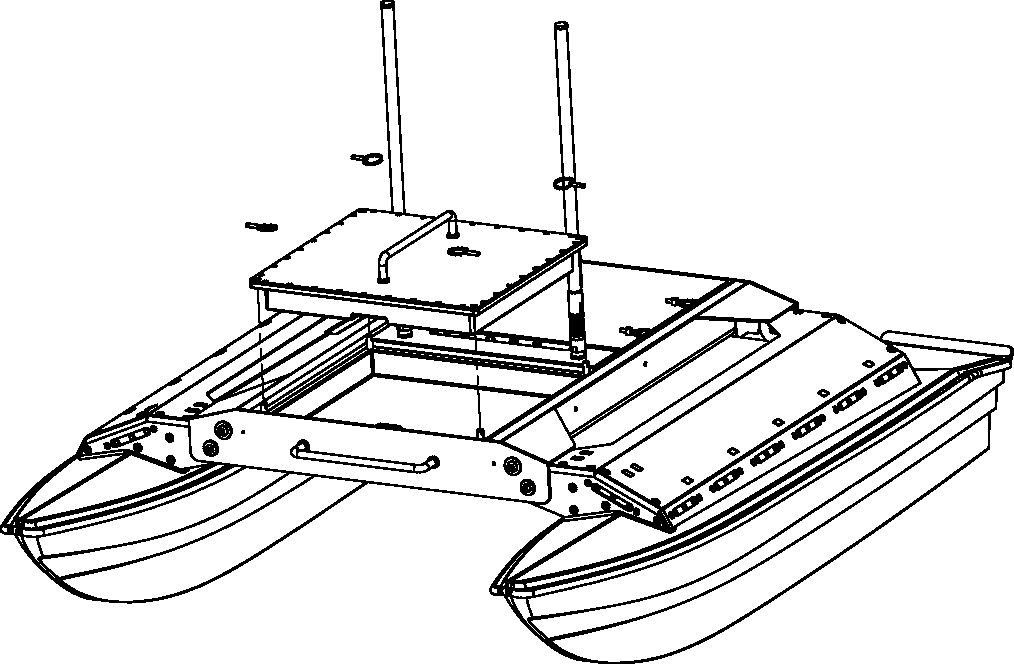
\includegraphics[width=0.75\linewidth]{graphics/h-battery.pdf}
  \caption{Battery Pack Insertion}
  \label{h_batteryinstall}
\end{figure}

\begin{enumerate}[nolistsep]
	\item Ensure Heron's main power button is in the outer “off” position.
	\item Carefully lower the Battery Pack. Ensure that it is firmly seated.
	\item Slide in the fast-pins into the battery retainers. It is OK if the battery retainers rotate, but do not allow them to unthread from their mounts.
	\item Plug in the Wet-Mate connector. Ensure there is adequate grease on the connector before attaching the battery to the boat.
\end{enumerate}
\textbf{Ensure that the battery is oriented correctly before lowering it into the Battery Bay.}

\begin{warning}
The Wet-Mate connector requires Molykote 44 grease. Ensure the connector is adequately greased each time before mating it to the boat or charger.
\end{warning}


The polarity of the battery pins for each of the two strings of NiMH cells is shown in \autoref{battery-pins} and \autoref{battery-pins-table}.

\begin{figure}[h]
  \centering
  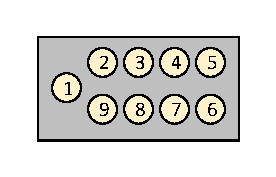
\includegraphics[width=0.5\linewidth]{graphics/h-batpin.pdf}
  \caption{Battery Pack Pinout}
  \label{battery-pins}
\end{figure}

\begin{table}[h]
\centering
\label{chg_pinout}
\begin{tabular}{|l|l|l|}
Pin number  & Function & Cable Wire Color \\
\hline
1  & unused & Black         \\ \hline
2  & +14V cell 1 & White  	\\ \hline
3  & +14V cell 1 & Red		\\ \hline
4  & GND cell 1 & Green     \\ \hline
5  & GND cell 1 & Orange    \\ \hline
6  & +14V cell 2 & Blue     \\ \hline
7  & +14V cell 2 & White/Black	\\ \hline
8  & GND cell 2 & Red/Black		\\ \hline
9  & GND cell 2 & Green/Black	\\ \hline

\end{tabular}
\label{battery-pins-table}
\caption{Subconn battery connector pinout}
\end{table}

\newpage

\subsection{Powering On}
To power on Heron firmly press the main power button. The power button light will illuminate, and a moment later, the running lights will come on solid for a few seconds before flashing. The motors will play a series of startup chirps to indicate ready status.

For R/C-only operation, the base station is unnecessary. However, if PC operation is required, set up and power-on the base station as well: Connect the battery to the power supply pigtail, and firmly press the button located on the side of the base station module. A blue LED in the power button will come on, and the radio inside the base station box will light up.

It may take Heron as long as five minutes to find the base station, but when it does, the flashing status indicator should move from Wireless Error (Slow Double Pulse) to No Command (Slow Single Pulse).

Before deploying into water, briefly test the activation of the Heron thrusters with the R/C controller and check wireless connectivity (if required). Do not run the thrusters out of water for more than a few seconds.

\subsection{Backup R/C Operation} \label{backupoperation}
Power-on the R/C controller. Flip the enable switch, top left corner (SW2), down toward the user, which puts Heron in manual override mode. This should be indicated by the Heron's running lights moving to short, Fast Single Pulses. Flipping the switch away from the user restores control to the onboard PC.

When operation of the thrusters has been verified on land, deploy Heron into the water and drive it around!

\subsection{Networking}

The Heron comes with a Microhard PX2 WiFi radio. The devices IP address is conventionally set to \textbf{192.168.131.10}.
The username and password to radio are:
\begin{itemize}
\item \textbf{username:} admin
\item \textbf{password:} clearpath
\end{itemize}


 The unit is supplied in the following configurations:

\begin{enumerate}
\item The PX2 is connected to the Clearpath network station as a client
\item the PX2 is configured as an access point and hosts its own network.
\end{enumerate}

To provide the USV access to the internet:

In configuration 1 with the PX2 configured as a client to the network station; connect the network station to your building's network by plugging in a LAN Ethernet cable to the station's Ethernet port. The Clearpath Network Station contains a second PX2 configured as an access point.

In configuration 2 with the USV PX2 configured as an access point:

\begin{enumerate}
\item \textbf{USB Adapter:}A USB to Ethernet Adapter can be used to wire your building's network to the robot. Plug this into the boat's USB port. This should give the robot access to the internet and allow anyone on the network to connect to the vehicle
\item \textbf{WiFi:} The vehicle's radio can be configured to connect to the building's WiFi as a client. Visit the radio's IP address 192.168.131.10, first download and save the default configuration and set the radio as a client to your WiFi network. Next change the radio to a client on your building's network. You will not be able to access the robot through the network, only through a local Ethernet connection.
\item \textbf{Ethernet:} The vehicle can be connected to the building's network via the Ethernet port. DHCP should first be disabled on the PX2 by visiting 192.168.131.1. Re-enable DHCP when complete.
\end{enumerate}



\newpage

\section{ROS Operation}
This section provides an overview of how to use ROS on Heron.

\subsection{PC Setup} \label{pcsetup}

To set up your workstation or laptop (hereafter “development machine”) to work with Heron, begin by following the setup instructions for ROS Kinetic: \url{http://wiki.ros.org/kinetic/Installation}.

Then, install the Heron ROS stacks:
(Note that many of the existing ROS packages, internet tutorials and support retain the Kingfisher nomenclature of the M200, these may be later updated to replace "kingfisher" with "Heron")

\begin{lstlisting}
sudo apt-get install ros-kinetic-heron-desktop
\end{lstlisting}

These packages can also be built from source if the package is not available from aptitude. Follow the ROS tutorials to create a catkin workspace. Visit \url{https://github.com/heron} and clone the heron desktop and heron packages to your workspace.

\url{http://wiki.ros.org/catkin/Tutorials/create_a_workspace}

Please contact Clearpath Robotics support if you have questions about upcoming functionality.



\subsection{SSH Connection}

\textbf{Note:} If you purchased a Basestation with your Heron USV, please refer to the accompanying Robotsmith Memo for instructions on how to connect to the embedded PC.

The embedded PC in Heron may be accessed directly, with a wired Ethernet cable, or over the wireless network created by the base station.

For wired access, use a standard Ethernet cable to connect from a laptop to the round Ethernet connector in the User Payload Area. Use your computer’s network configuration utilities to give your Ethernet port an IP in the 192.168.131.x subnet. For example, from the Ubuntu commandline:

\begin{lstlisting}
sudo ifconfig eth0 192.168.131.5 up
\end{lstlisting}

Now attempt to ping the onboard computer at its standard IP:

\begin{lstlisting}
ping 192.168.131.1
\end{lstlisting}

If successful, you should be ready to connect:

\begin{lstlisting}
ssh administrator@192.168.131.1
\end{lstlisting}

The default password is \lstinline{clearpath}.


\textbf{For wireless access}, connect to the base station’s LAN port with an Ethernet cable, or simply join the wireless network (use the credentials included with your shipment).

\textbf{To configure the wireless network settings}, configure the Heron WiFi radio's settings by visiting 192.168.131.10 in your browser while wired to the vehicle or connected to the wireless network.


To give Heron access to the Internet, connect the base station’s WAN port to a wired network connection, or configure the WiFi radio to temporarily connect Heron to a wireless network with Internet access (such as a wireless hotspot).

\subsection{Developing with the Onboard PC}
When connected to the onboard PC via SSH, be aware of the following locations:

\begin{itemize}[nolistsep]
	\item \textbf{/opt/ros/kinectic} is where ROS packages from apt live, including Heron’s core packages. You should not need to modify the contents of this directory.
	\item \textbf{/etc/ros/kinetic/ros.d} is a directory of roslaunch files which are launched on bootup of Heron's computer.
\end{itemize}

When you are ready to develop additional software to add to Heron, the recommended path is to add your source repo to a new \lstinline{~/catkin_ws overlay} . When you roslaunch your software, it will seamlessly connect to the already-running background ROS network.

When you’re ready to launch some of your software on boat startup, you can add launchfiles to the \lstinline{ros.d} path, but you will also need to change the workspace sourced by the background job. To do this, edit the final line of the \lstinline{/etc/ros/setup.bash} file, and set it to source the setup.bash of the workspace containing the packages which your startup launch file will require.

For more information on using Overlays, see the ROS wiki: \url{http://wiki.ros.org/catkin/Tutorials/workspace_overlaying}

\subsection{ROS Remote Setup}
Connecting with SSH provides a first approach to connecting with the vehicle, however, users often want to be able to run ROS nodes on their development machine and have them able to communicate with the vehicle. This is especially the case with nodes which have a desktop visualization component, such as \lstinline{rviz} or \lstinline{image_view}, or when you want to interface with a locally-connected peripheral, such as the game controller.

The nodes which are launched on startup of Heron have the following environment set:

\begin{lstlisting}
export ROS_IP=192.168.131.1
export ROS_MASTER_URI=http://$ROS_IP:11311
\end{lstlisting}

When connecting to Heron via the wired Ethernet port, with an IP such as 192.168.131.5 (as instructed above), the setup of the environment on your workstation is indeed simple:

\begin{lstlisting}
export ROS_IP=192.168.131.5
export ROS_MASTER_URI=http://192.168.131.1:11311
\end{lstlisting}

Once these two commands have been executed on your workstation, it should be possible to run \lstinline{rostopic list, rostopic echo,} etc. to verify that you are communicating with the onboard roscore.



\subsection{ROS Remote Teleoperation}

When the developer machine has been correctly configured for remote ROS, it will be possible to install the ROS teleop twist joy package, plug in a standard USB joystick and launch Heron teleoperation:

\begin{lstlisting}
roslaunch teleop_twist_joy teleop.launch
\end{lstlisting}

This will launch, locally on the development machine, the standard ROS joystick driver, and a translation node which converts joystick messages into velocity command messages. Hold button 1 on your joystick to enable command messages to be sent.

Note that this package is currently being transitioned from legacy Kingfisher packages. Please contact Clearpath support if any issues arise.

\pagebreak

\subsection{Key Topics}
Heron ships with a suite of standard hardware. Each included peripheral is set up from the get-go with appropriate driver software on the onboard PC. This section details how to find the various topics related to each device.

When connected via SSH, or by setting up remote ROS (as detailed above), list available topics with:

\begin{lstlisting}
rostopic list
\end{lstlisting}

The \textbf{drive system} publishes information about battery voltage and motor current on the \lstinline{/sense} topic. It listens for commands on \lstinline{/cmd_drive} (kingfisher\_msgs/Drive).

The \textbf{IMU} publishes data on the \lstinline{/imu/data} topic.

The \textbf{GPS} publishes fixes on the \lstinline{/navsat/fix} topic.

Information from the MCU is available on the \lstinline{/sense} topic.

\subsection{Compass Calibration}

To calibrate the magnetometer on the IMU, place the Heron in open water and run the calibrate compass script. The boat will turn in place while it takes measurements from the magnetometer for 60s. It will then save a configuration file for the compass which will be used when the vehicle powers on. Ensure that the configuration YAML file is saved to the proper working directory of the Heron packages:\texttt{heron\_base/config/imu\_compass.yaml.}

\begin{lstlisting}
\texttt{rosrun heron\_bringup calibrate_compass}
\end{lstlisting}

\subsection{NMEA Interface}

The Heron has an NMEA interface available for use with software packages such as MOOS-IVP. By default, the NMEA interface is not configured to run on launch. To start the NMEA interface automatically on launch, add the nmea\_if.launch file to the startup launch directory ( /etc/ros/kinectic/ros.d) , or install it with the robot\_upstart package.
\begin{lstlisting}
sudo cp \texttt{/opt/ros/kinectic/share/heron_nmea/launch/nmea_if.launch /etc/ros/kinectic/ros.d/}
\end{lstlisting}

\newpage

\section{Payload Integration}
The User Payload Area of Heron includes a standard Ethernet connector, 3 USB connectors and 2 custom RS232 + 12V power connectors. These may be used to power and communicate with payloads such as sonar-based instruments, LiDARs and cameras.

\textbf{When the mating connectors are not being used the supplied plug connector and dust cap must be installed to ensure that the Heron electronics remain sealed.}

The waterproof ethernet panel connector on the Heron electronic enclosure is part number \textbf{RR-225200-30} available from www.USBfirewire.com. The mating connector can be either part number \textbf{RR-225360-00} - RJ45 Field Installable Conenctor or \textbf{RR-225320-06-XX} RJ45 Waterproof Cable, also available from www.USBfirewire.com



\begin{figure}[h]
  \centering
  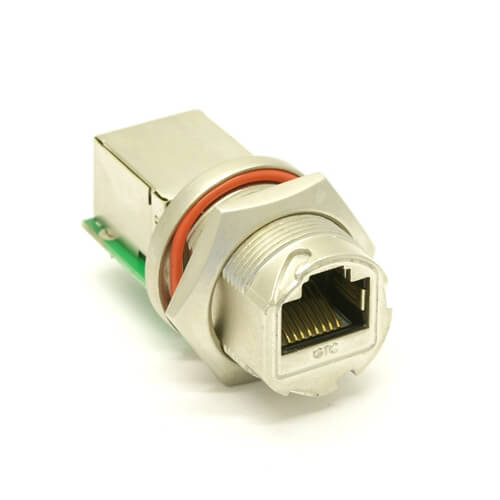
\includegraphics[width=0.25\linewidth]{graphics/RR-225200-30.jpg}
  \label{h_eth0}
  \caption{Electronics Enclosure Ethernet Connector}
\end{figure}

\begin{figure}[h]
  \centering
  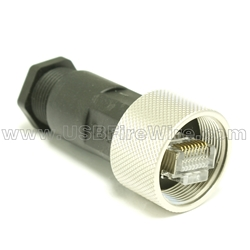
\includegraphics[width=0.25\linewidth]{graphics/RR-225360-00.jpg}
  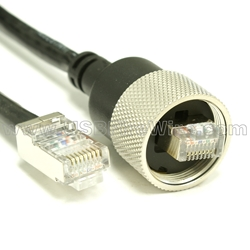
\includegraphics[width=0.25\linewidth]{graphics/RR-225320-06-118.jpg}

  \label{h_eth1}
  \caption{Electronics Enclosure Ethernet Connection options RR-225360-00 and RR-225320-06-XX}
\end{figure}

The mating connector for the waterproof USB panel mount connectors RR-218300-30 on the Heron electronics enclosure bay is part number \textbf{RR-116370-00} -field installable connector from USBfirewire.com. Please review other mating options for the screw-lock type USB connectors available on usbfirewire.com such as \textbf{RR-116320-06-39} - Waterproof USB Cable - A Extension.

\begin{figure}[h]
  \centering
  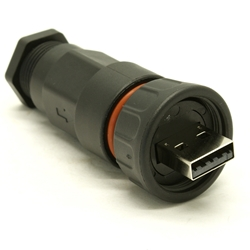
\includegraphics[width=0.25\linewidth]{RR-116370-00.jpg}
  \label{h_usb0}
  \caption{Electronics Enclosure USB connector RR-116370-00}
\end{figure}

RS232 and 12V power are supplied via two female panel mount Chogori Standard Series 6-pin connectors on the Heron electronics enclosure (part number \textbf{22006615-01}).  The mating connector is a Chogori 6-pin male cord plug, part number \textbf{22006111-01} . Please review the data sheets of each connector prior to assembly. The pin-out for the mating Chogori cord connector is given in \autoref{chg_pins} and \autoref{chg_pinout}. Note that \autoref{chg_pinout} should be interpreted as viewed from the solder end of the field installable connector.

\begin{figure}[h]
  \centering
  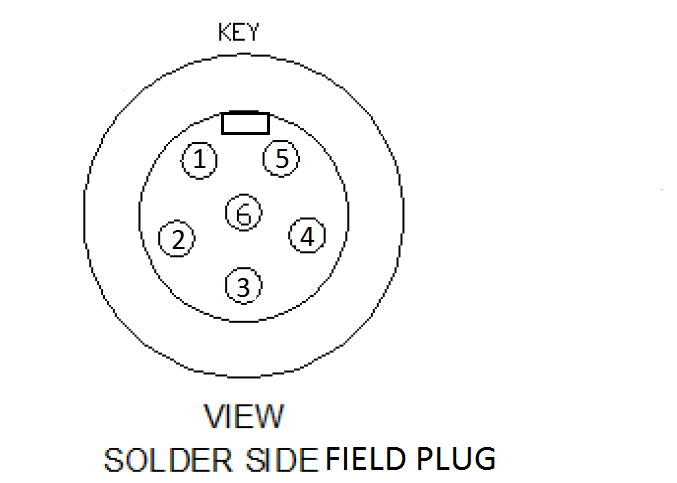
\includegraphics[width=0.5\linewidth]{graphics/h-field_conn_pins.png}
  \label{chg_pins}
  \caption{Chogori Field Installable Connector pin numbering }
\end{figure}


The pinout for this connector is as follows:


\begin{table}[h]
\centering
\label{chg_pinout}
\begin{tabular}{|l|l|}
Pin number  & Function \\
\hline
1  & GND              \\ \hline
2  & TX  \\ \hline
3  & RTS  \\ \hline
4  & 12V Supply            \\ \hline
5  & RX             \\ \hline
6  & CTS            \\ \hline

\end{tabular}
\caption{EN3 Pin Function}
\end{table}

The RS232 ports are available on the on-board PC as devices: \textbf{ttyS4} \textbf{ttyS5}. These ports may not function if the BIOS of the PC have been reset to factory default.

\newpage

\section{Maintenance}
Heron is built for rugged, long-term use. However, there are steps that can be taken to maintain and extend the life of the platform even further.

\subsection{Charging}
The Battery Pack which ships with Heron can be charged with the following steps:

\begin{enumerate}[nolistsep]
	\item Remove Battery Pack from platform.
	\item Connect the SubConn Wet-Mate output adapter cable from the charger to the Battery Pack terminal connector. Ensure the connector has adequate Molykote 44 grease
	\item Configure the charger to charge both sells on the NiMH setting at 2amps.
	\item Begin charging with each channel of the charger. The charger will report the battery voltage and charging current. The charger will automatically stop when each channel has reached full charge at approximately 17V.
\end{enumerate}

\begin{warning}
The Heron battery pack contains 2, 14V, 14.5Ah strings of NiMH batteries. Ensure each channel of the charger is activated when charging the battery.
\end{warning}

\begin{warning}
Do not plug a battery pack with unbalanced cells into the Heron.
\end{warning}

\subsection{Battery Pack}
Heron's power supply is a sealed 14.4 V nickel metal hydride (NiMH) battery, providing 29 ampere-hours of charge. To maximize the lifetime of the Battery Pack, recharge immediately after use, and keep charged to prevent loss in capacity.

The Battery Pack should never be used or stored in an environment exceeding 40 degrees Celsius (104 °F), and should always be charged at temperatures above freezing.

\subsection{Electronics Bay}
Heron's electronics are enclosed in a sealed compartment. These do not require maintenance, and the bay should only be opened by, or under the supervision of, Clearpath Robotics.

\newpage

\section{Operator Checklist}

\begin{enumerate}
\item Ensure all batteries are charged: vehicle battery, RC remote battery, base station battery. The vehicle battery voltage is visible on the RC remote at close range.
\item Ensure all fittings and connectors are not loose. These include: antenna connectors, USB, Ethernet and RS232 connectors, thruster and LED connectors.
\item Ensure all connector caps or payload connections are attached.
\item Ensure the WiFi is connected if required.
\end{enumerate}

\newpage

\section{Tips and Troubleshooting}
This section lists a few possible issues which may be encountered in the course of using Heron.

\bgroup
\def\arraystretch{1.5}%
\begin{table}[h]
\centering
\label{troublshooting}
\begin{tabular}{p{.2\textwidth} p{.7\textwidth}}

\rowcolor{lightgrey}
{\bf Observation}                    & {\bf Issue \& Resolution}                                                                                                                                                                                                                                                                                          \\ \hline
No power LED                         & \textbf{System is unpowered}. Ensure power button is pressed, and check that battery is properly seated in battery bay. It is unlikely that the battery would be so discharged as to be unable to illuminate the LED, but you could also confirm with a multimeter that the battery has a terminal voltage of at least 14V. \\ \hline
Running lights indicate error status & \textbf{System is in error}. Please refer to Status Indicators on page \pageref{statusindicators} to determine the status being indicated, and contact support for further assistance.                                                                                                                                                               \\ \hline
Can’t ping onboard PC                & \textbf{Network problem}. Ensure that Heron is indicating successful connection to the base station, and that the user laptop is also successfully connected (ie, able to ping 192.168.131.9).                                                                                                                           \\ \hline
Unable to list ROS topics            & \textbf{ROS network problem}. Ensure that the user laptop has a working ROS installation, including the Heron workspace. Ensure that ROS\_MASTER\_URI is correctly pointing to the Heron IP, and that ROS\_IP is set to the user laptop’s IP.                                                                     \\ \hline
Unable to echo ROS topics            & \textbf{ROS environment problem}. Ensure that the user laptop is able to ping Heron, and that ROS\_MASTER\_URI and ROS\_IP are set correctly.                                                                                                                                                                          \\ \hline
\end{tabular}
\end{table}
\egroup

If you’re having some trouble that you don’t see here, or the suggested solution isn’t working out, please get in touch so we can help you with it (see next page for contact details).

For more details on setting up multiple machines to work together in ROS, please see the following pages on the ROS wiki:

\begin{itemize}[nolistsep]


	\item \url{http://www.ros.org/wiki/ROS/NetworkSetup}
	\item \url{http://www.ros.org/wiki/ROS/Tutorials/MultipleMachines}
\end{itemize}

\newpage

\section{Service and Support}
Clearpath is committed to your success with Heron. Please get in touch with us and we'll
do our best to get you rolling again quickly: \href{mailto:support@clearpathrobotics.com}{support@clearpathrobotics.com}
or visit out knowledge base for at \href{http://support.clearpathrobotics.com}{support.clearpathrobotics.com}

To get in touch with our sales team regarding Heron or other Clearpath Robotics products, please
email \href{mailto:sales@clearpathrobotics.com}{sales@clearpathrobotics.com}.

If you have a an issue that is specifically about ROS and is something which may be of interest
to the broader community, consider asking it on \href{http://answers.ros.org}{answers.ros.org}.
If you don't get a satisfactory response, please ping us and include a link to your question
as posted there. If appropriate, we'll answer in the ROS Answers context for the benefit of the
community.

\end{document}
